%
% zyklus.tex
%
% (c) 2021 Prof Dr Andreas Müller, OST Ostschweizer Fachhochschule
%
\documentclass[tikz]{standalone}
\usepackage{times}
\usepackage{amsmath}
\usepackage{txfonts}
\usepackage[utf8]{inputenc}
\usepackage{graphics}
\usetikzlibrary{arrows,intersections,math}
\usepackage{ifthen}
\begin{document}

\newboolean{showgrid}
\setboolean{showgrid}{false}
\def\breite{7}
\def\hoehe{4}
\def\beschriftung{
\node at (-2,-1.4) {$a$};
\node at (1.45,-2.6) {$b$};
\node at (1.8,-0.8) {$c$};
\node at (-0.8,2.3) {$d$};
}
\begin{tikzpicture}[>=latex,thick]
\clip (-6.3,-3.27) rectangle (6.3,3.27);

% Povray Bild
\begin{scope}[xshift=-3.2cm]
\node at (0,0) {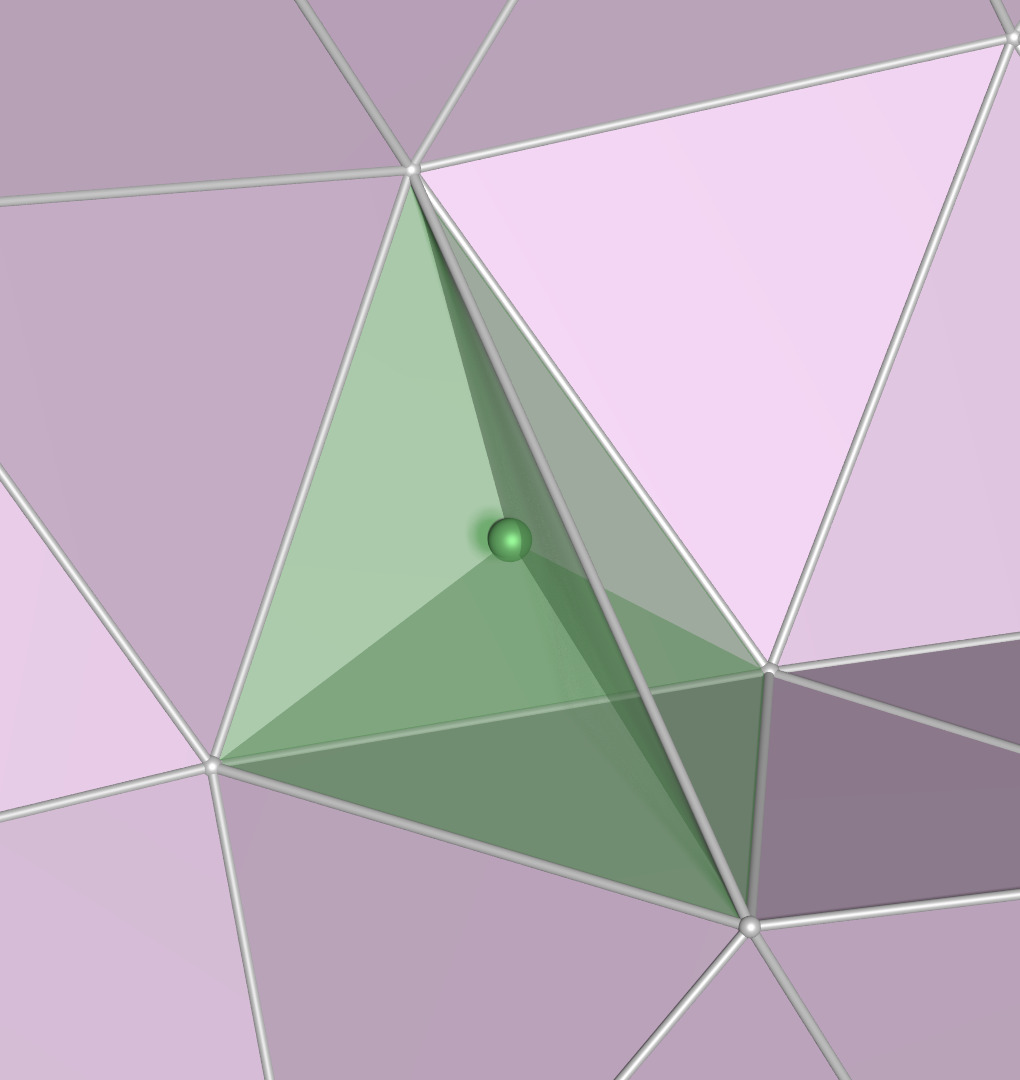
\includegraphics[width=6.2cm]{zyklus.jpg}};
\beschriftung
\node at (-0.3,0) {$p$};
\end{scope}

\begin{scope}[xshift=3.2cm]
\node at (0,0) {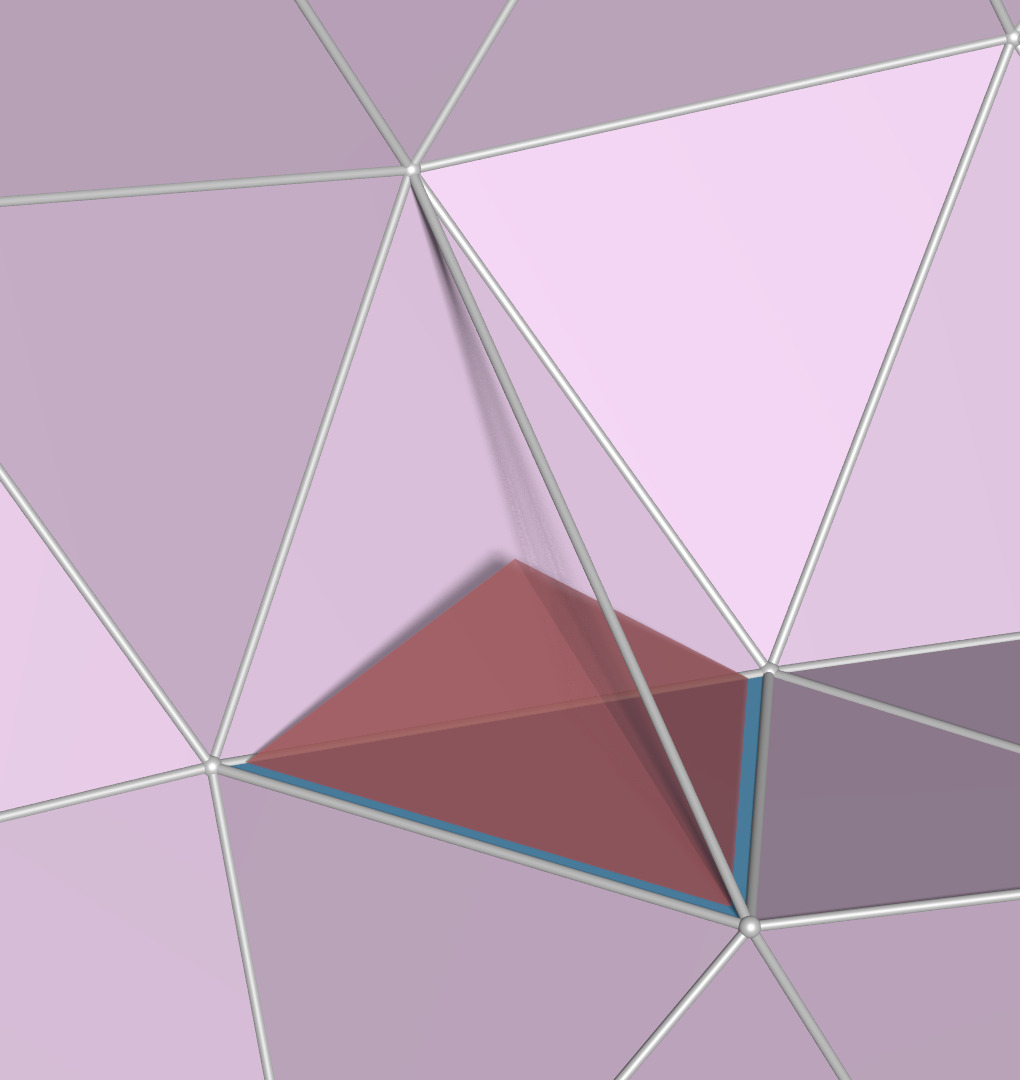
\includegraphics[width=6.2cm]{zhomolog.jpg}};
\beschriftung
\node at (-0.0,0.1) {$p$};
\end{scope}

% Gitter
\ifthenelse{\boolean{showgrid}}{
\draw[step=0.1,line width=0.1pt] (-\breite,-\hoehe) grid (\breite, \hoehe);
\draw[step=0.5,line width=0.4pt] (-\breite,-\hoehe) grid (\breite, \hoehe);
\draw                            (-\breite,-\hoehe) grid (\breite, \hoehe);
\fill (0,0) circle[radius=0.05];
}{}

\end{tikzpicture}

\end{document}

